% \IEEEraisesectionheading{
%     \section{Introduction}
%     \label{sec:introduction}
% }
\section{Introduction}
\label{sec:introduction}
%NOTE: (1) MEC Introduction: Background, Challenge and Motivation
%NOTE: (1a) general background and bluffing
\IEEEPARstart{E}{dge} computing is gaining more and more attention with the prosperity of computation-intensive and delay-sensitive mobile applications. % computation-intensive, energy-hungry
The edge servers are deployed in closer proximity to mobile IoT devices than the traditional cloud computing infrastructure, which enable computation offloading from mobile IoT devices (e.g., mobile phones, video surveillance cameras, etc.) via Access Points (APs) and alleviate the communication overhead. 
%NOTE: (1b) why multiple edge servers deployed
Since the edge servers are usually with limited computation resources, the distributed deployment of edge computing servers in the network is favored.
Therefore, a fundamental problem in edge computing is to investigate the cooperative job dispatching among multiple APs and edge servers as illustrated in Fig.\ref{fig:system}.
% Hence, it is necessary to investigate the cooperative job dispatching among multiple APs and edge servers, \hongyc{as illustrated in Fig.\ref{fig:system}.}
More specifically, mobile IoT devices offload jobs through APs, each of which performs as a job dispatcher to choose edge servers processing the data. Typically, there are a large number of APs in a Metropolitan Area Network (MAN). Some APs are co-located with edge servers while others are not. %Edge servers are deployed with some APs and the index number is same for the collocated AP and edge server as illustrated in Fig.\ref{fig:system}}
%\tann{AP \& Edge servers \& dispatcher, a figure preferred?}
%\tann{AP collect information, and performs as a dispatcher.
%dispatch to an edge server, which is deployed with some APs.}

\begin{figure*}[htp!]
    \centering
    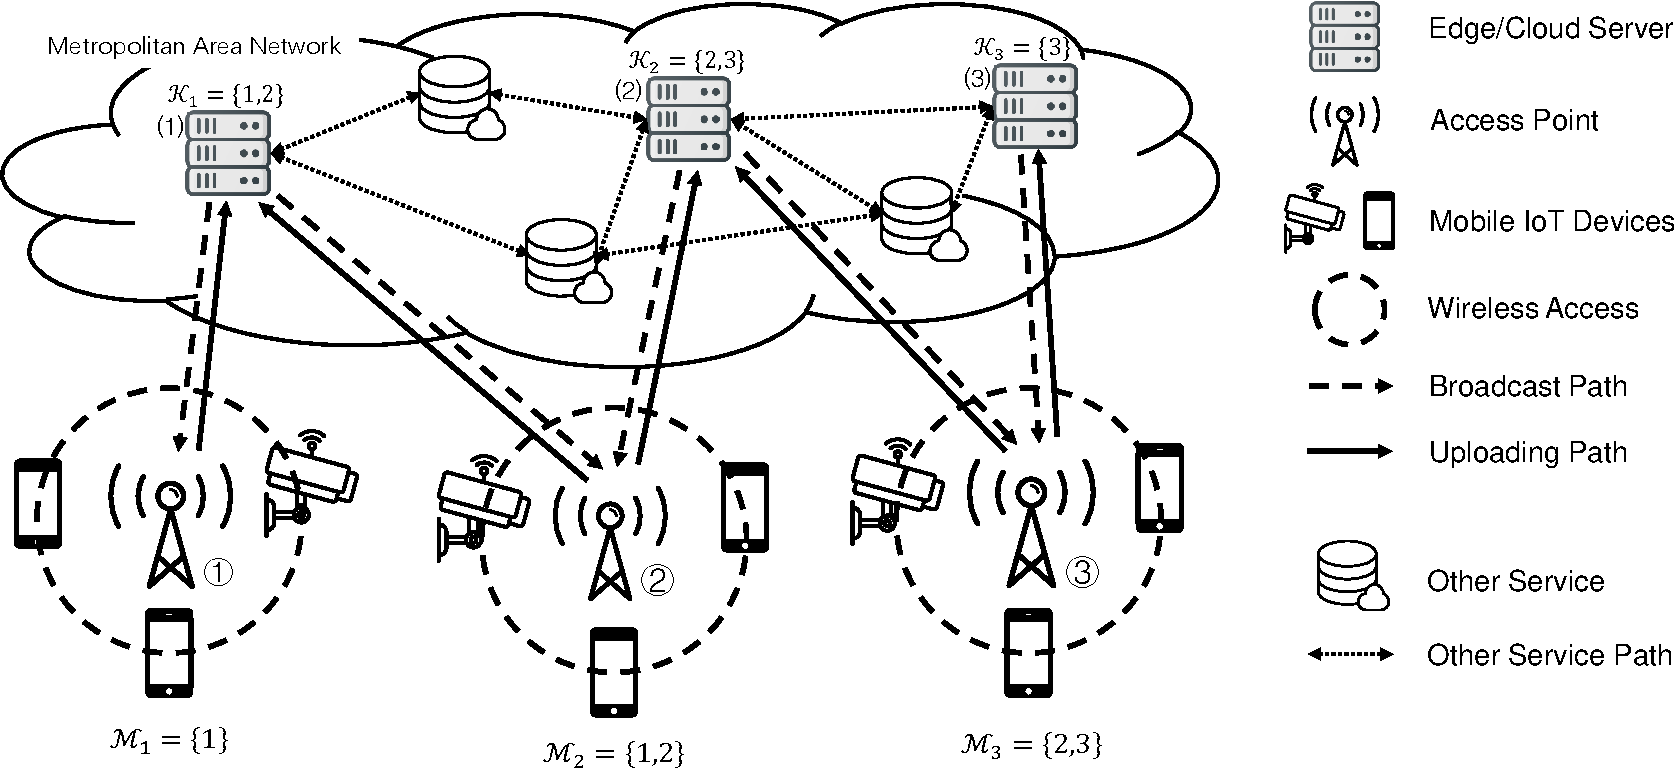
\includegraphics[width=0.60\textwidth]{system-model.pdf}
    \caption{The Illustration of System Model.}
    \label{fig:system}
\end{figure*}

% In a general edge-cloud system architecture \cite{MEC-SURVEY}, the offloaded jobs from {IoT devices} could be delivered to one of the edge servers considering the transmission latency, job processing time, back pressure and etc.
%NOTE: (1c) introduce the access points
% The entity which decides edge servers for offloaded jobs is called \emph{access points} (APs) throughout this paper.
% Specifically, the APs function as gateways to collect offloaded jobs from {mobile IoT devices} in its service area and make dispatching decision for each job.

%NOTE: (2) Motivation with MAN and Distributed Dispatchers
%NOTE: (2a) why cooperation is needed; cooperation in MAN is another challenge
% To achieve better overall performance (e.g., average job response time) of the edge computing system, the cooperation of jobs dispatching among distributed APs is one of the major challenges.
Most existing works assume a centralized job dispatcher, which has timely and complete knowledge of the global system status and distributes the dispatching decisions to all the APs without delay \cite{tan-online,IOTJ18-FanQ,mdp-globecom,mdp-tvt,MASS18-MengZ}.
However, the edge computing systems are usually deployed at Metropolitan Area Network (MAN) scale in practice, e.g., the Edge Computing Interconnect (ECI) Network \cite{MAN-ECI}, where the latency of information sharing among APs and edge servers is non-negligible. Moreover, according to the MAN performance analysis in \cite{MAN-LATENCY}, the end-to-end transmission latency is highly variable with respect to different hours of the day and IoT devices' locations in a MAN, which implies the randomness in the job uploading latency from APs to edge servers as well as the signaling latency (i.e., the transmission latency of the {system status} information).
%NOTE: (2b) challenge brought by random latency
There have been several works in the literature considering random transmission latency of job delivery in the edge computing network \cite{latency-EDGE19,MOBIHOC19-ZhouZ,IOTJ18-FanQ,TOC19-LiuC,JSAC19-AlameddineHA}.
However, there are few works considering the random signaling latency of information sharing among distributed dispatchers \cite{tan-online,TWC18-LyuX}.
In fact, it is full of \revision{challenges} to consider random transmission latency in both job uploading and signaling in edge systems.
\hongycCHK{
\begin{itemize}
    % 1) signaling latency: centralized/distributed, outdated information
    \item Firstly, the centralized dispatcher design is discouraged for unpredictable signaling latency, as the distribution of dispatching decisions would consume extra random time. For distributed dispatchers design, the information exchange among distributed dispatchers also suffers from significant signaling overhead and outdated information.
    %Firstly, the centralized dispatcher is discouraged for outdated system information and unpredictable signaling latency.
    % 2) uploading latency: inconsistency information exchange;
    \item Secondly, as the job arrivals at edge servers are unknown in advance because of random uploading latency, different dispatchers would have inconsistent system information even if the signaling latency is fixed.
    % Secondly, the random uploading latency causes the inconsistency of system information at different dispatchers because the job arrivals at edge servers are unknown in advance.
\end{itemize}
}

To conclude, the random transmission latency may introduce ineliminable estimation errors on the number of jobs at APs or edge servers in the system.
% {i.e., the cooperation of APs are assumed inside one entity like a operator, but across a large network which is larger than a LAN.}
% {In addition, each AP also suffers from signaling latency, which is the time consumed for each AP to collect system state information under some signaling mechanism.}


% NOTE: (3) Our contributions
In this paper, we address the above challenges by leveraging a partially observable Markov decision process (POMDP) problem formulation, and a novel low-complexity approximate MDP solution framework is proposed.
Specifically, we consider a practical scenario where the APs cooperatively upload different types of jobs to different edge servers with random uploading latency, and the APs receive the partial system state information suffering from random signaling latency (i.e., the global system state is always partially available and outdated at the APs).
The major contributions in this paper are summarized below.
\begin{itemize}
    \item The distributed and cooperative job dispatching design with outdated and partial information is formulated as a POMDP problem.
    Different from the conventional value or policy iteration of the Bellman's equations where global or historical system states are requested in numerical calculation, a novel low-complexity approximate MDP solution framework via \emph{alternative policy iteration} is proposed, where the dispatching policies of all APs are updated distributedly and alternatively based on the {closed-form expression} of the approximate local value function.
    Thus, the conventional complicated POMDP solution is avoided.
    % {where each AP collects the information only from the APs and edge servers in close proximity and make dispatching decisions with random signaling latency.}
    % {we directly derive the expression of approximate value function}
    \item Both analytical performance lower bound and tighter semi-analytical lower bound are derived for the proposed distributed dispatching policy. In the conventional approximate MDP methods, the performance is usually evaluated numerically.
    The lower bounds not only justify the reliability of the proposed policy but also provide a method of quick performance evaluation.
    \item We extend our solution framework \algname~with an efficient online learning approach to evaluate the approximate value function when the priori knowledge of the system randomness is absent.
    \item We conduct extensive simulations based on the Google Cluster trace, compared with three heuristic benchmarks. The evaluation results show that \algname~can achieve as high as $20.67\%$ reduction in average job response time and consistently perform well under various parameter settings of signaling latency, job arrival intensity and job processing time. {Moreover, the online learning algorithm converges fast.}
    %\tann{show some number of performance gain. e.g., xxx$\times$, xxx\% }
\end{itemize}

% The extended \algname~could converge to the real parameter settings fast with negligible error

The remainder of this paper is organized as follows.
In Section \ref{sec:review}, we introduce some related works about job scheduling in edge computing systems.
In Section \ref{sec:model}, we elaborate the system model and the signaling mechanism with random transmission latency.
In Section \ref{sec:formulation}, we formulate the global-wise optimization of dispatching decisions at all APs as a POMDP.
In Section \ref{sec:algorithm}, we propose a novel low-complexity approximate MDP solution framework, called \algname.
% where the policy iteration could be applied distributedly on each AP {with partial and outdated information}.
In Section \ref{sec:rl-alg}, the solution framework is extended with reinforcement learning technique to handle the unknown statistics.
The numerical analysis of the proposed solution is provided in Section \ref{sec:evaluation}, and the conclusion is drawn in Section \ref{sec:conclusion}.

We use the following notations throughout this paper: 
non-bold letters (e.g., $a, A$) are used to denote scalar values,
bold lowercase letters (e.g., $\mathbf{a}$) are used to denote column vectors,
bold uppercase letters (e.g., $\mathbf{A}$) are used to denote matrices,
and calligraphic letters (e.g., $\mathcal{A}$) are used to denote sets.
Using these notations, $\mathcal{A}\backslash\mathcal{A'}$ denotes set subtraction of $A'$ from $A$; $[\mathbf{A}]_{i,j}$ and $\mathbf{A}'$ denotes the $(i,j)$-th element and transpose of matrix $\mathbf{A}$, respectively.
% $\mathbf{I}$ denotes the identity matrix.

\section{Related Works}
\label{sec:review}
%NOTE: (1) resource placement (cache-like problem), service migration
There have been a number of works aiming at reducing job response time by resource allocation and service migration in the edge computing system.
For example, in \cite{TON19-WangSq}, the edge servers are one-to-one bound to the base stations (BSs), and the job migration could be applied according to users' mobility traces via the backhaul network connecting the BSs.
However, according to a recent research \cite{INFOCOM19-WuC}, the resource re-allocation for running jobs on servers is hard to implement in practice, as it is hard for jobs migration among heterogeneous edge servers with different resource configurations.
Hence, it could be more important to optimize the job dispatching strategy at their arrival time.

%NOTE: (2) single-agent job dispatching, single UE/server
There also have been a number of works considering centralized job dispatcher design with timely and complete knowledge of the system status.
For example, in edge computing systems with fixed uploading latency, the authors in \cite{tan-online} designed an online algorithm to minimize the average job response time in the worst case.
In the scenario that BSs and edge servers are connected via software defined network (SDN), the authors in \cite{IOTJ18-FanQ} proposed a heuristic algorithm to dispatch the jobs to the closest edge servers according to geographical locations.
Considering random jobs arrival, the authors in \cite{mdp-globecom,mdp-tvt} formulate the offloading design to a single edge server as an infinite-horizon Markov decision process (MDP).
When the jobs can be dispatched to either edge servers or cloud servers, the authors in \cite{MASS18-MengZ} formulated the job dispatching problem as integer linear programming to minimize the total uploading latency. % with fixed uploading latency
% In the above works, a centralized dispatcher with complete and instant knowledge of the system status was assumed in the edge computing systems, which might be impractical.

%NOTE: (3) multiple-agent job dispatching
Since centralized dispatching design might not be suitable for \revision{edge computing systems} with distributed deployment, there are also some works addressing the distributed job dispatching.
For example, in order to minimize a weighted sum of total energy consumption and uploading latency, the authors in \cite{ToN-Xuchen2016} proposed a distributed job dispatching algorithm based on game theory to achieve the Nash equilibrium. 
Considering job migration at edge servers, the authors in \cite{ToN-xujie2018} optimized the edge computing performance in a distributed manner with limited energy resources via a congestion game framework.
In a scenario that APs cooperatively dispatch jobs with multiple edge servers, the authors in \cite{mdp-jcin} proposed \revision{an} approximate MDP method to alleviate the computational complexity and minimize the average job response time.
However, in the above works, the latency of information exchange among APs and edge servers is ignored.
In fact, due to the complicated network traffic, this latency might be significant, and the staleness {and failed transmission} of system state information at the dispatcher of edge computing systems should be considered.

%NOTE: (4) stale-information based multi-agent related works
%TODO: (Optional) if have time, rewrite this part
The staleness of information sharing among APs and edge servers may degrade the performance of the job dispatching algorithm in edge computing systems.
To the best of our knowledge, there are very limited works investigating this issue.
The authors in \cite{JSAC17-LyuX} proposed a randomized policy via Lyapunov optimization approach to stabilize the queues in a MEC system with multiple IoT devices offloading jobs to one edge server, where \brlatency~is considered. 
In \cite{TWC18-LyuX}, the above approach was applied to the scenario that mobile devices offload jobs to each other via D2D link.
In the above two works, there is one centralized dispatcher in the system, and the objective is to stabilize the transmission queues.
Hence, the existence of \brlatency~may not raise a significant challenge to the algorithm design with Lyapunov optimization.
In fact, the design of distributed dispatchers with \brlatency~could be more challenging.
For example, the signaling latencies at distributed dispatchers could be different, and the synchronization of their dispatching decisions becomes infeasible.
Furthermore, taking the signaling overhead and the possibility of packet drop revision{into} consideration, it is of more practical favor to make scheduling decisions based on locally observable system state information, instead of global system state information.
To our best knowledge, there is no appropriate optimization framework for the distributed dispatcher design with both \brlatency~and partially observable system state information to date.

%----------------------------------------------------------------------------------------%
